% CAPÍTULO 18 — «O instrumento mexe no mundo» (a travessia C×D, a pergunta com realimentação)
% Fracasso que o abre: o vigia chega quando \numVigiaTomboRecentePagoPct\% do prejuízo já está pago
% (cap. 4), a resposta natural é agir no disparo --- e agir muda o mundo que o vigia lê.
% Ancoras: numVigiaTomboRecentePagoPct (cap. 4), numSerieDias, numPromessaPct, numCortePosto;
% novo: caderno E35_performativos (semente 101, \numLacoMundos{} mundos, laço com fração e atraso).
% Figuras: figuras/E35_performativos_1.pdf (entrega ciclo a ciclo, atraso zero) e
% figuras/E35_performativos_2.pdf (o preço pareado por mundo).
% Costuras: o fecho do capítulo da partilha abre esta porta; o nosso fecho entrega a conta do
% esquecer ao capítulo da memória que aprende.

\chapter{O instrumento mexe no mundo}\label{cap:instrumento}

\section{A decisão que o próprio livro adiou}

O capítulo do orçamento do alarme mediu o preço de chegar tarde: quando o vigia finalmente apita,
\numVigiaTomboRecentePagoPct\% do prejuízo já foi pago. A resposta natural cabe numa linha --- agir
no disparo, vender antes que o resto do tombo chegue --- e é aí que a medição muda de lado: agir
muda o mundo que o vigia lê. A venda devolve parte da oscilação ao dia seguinte; o dia seguinte,
mais leve, alimenta a janela que ergue o corte; o corte novo decide a próxima venda. O instrumento
deixou de olhar o mundo e passou a conversar com ele.

Todo o livro mediu até aqui num mundo que não olha de volta. A promessa do corte, o piso do
orçamento, a partilha do relógio: barreiras erguidas sobre séries que seguiam o seu sorteio
independentes de quem as media. O capítulo da partilha fechou no limite honesto --- a escala é a
que precisa ser atualizada sempre --- e deixou a frase que este capítulo pega no bolso: atualizar
é uma decisão sobre o mundo, e ninguém mediu o que essa decisão faz com a própria medida. A
pergunta tem nome na literatura \cite{perdomo2020performative} e tem controle na casa: medir é
família declarada, e o laço que a família produz é medição, não mercado.

Duas leituras cabem, e elas não dão a mesma resposta. Se o laço for contrátil, a barreira
recalibrada converge para um ponto em que a entrega volta a valer a promessa --- mas com outro
corte, porque o instrumento apertou o mundo em vez de medir o risco. Se não for, a entrega anda de
ciclo a ciclo, e o que a partilha mediu como orçamento passa a ter um termo que ninguém declarou.
A diferença entre as duas é a medição deste capítulo.

\section{O laço, declarado}

O mundo é o da casa: \numSerieDias{} dias de nível estável, um sorteio por mundo,
\numLacoMundos{} mundos, tudo reportado com a dispersão entre eles. O corte é o da raiz, o
\numCortePosto{}º pior da janela de um ano. A ação é declarada e tem dois parâmetros de topo: a
fração da posição vendida a cada rompimento, e o atraso entre o rompimento e a venda --- vender no
próprio dia do rompimento, no dia seguinte, ou cinco dias depois. Vendida a fração, o retorno
realizado do dia da venda vem amortecido: é essa a parte da oscilação que a ação devolve.

A recalibragem é o laço: o corte é refeito a cada ciclo sobre a série que o ciclo anterior produziu
--- a série com as vendas dentro ---, cinco ciclos, nada de peça nova \cite{mendlerdunner2020stochastic}.
E antes de qualquer número, o controle: fração nula, a venda que não acontece. O laço com reação
nula tem de devolver o mundo intacto, dia por dia, e a calibragem parada --- é o controle da
transformação neutra \cite{ng1999policy}, e ele passa: as séries voltam bit a bit, os cortes não
andam, e a entrega mediana fica em \numLacoEntregaNulaMedianaPct\%, contra os
\numLacoPromessaAssinadaPct\% que o corte assina. É o controle que separa o resto.

\section{A entrega no mundo que reage}

\begin{figure}[ht]
\centering
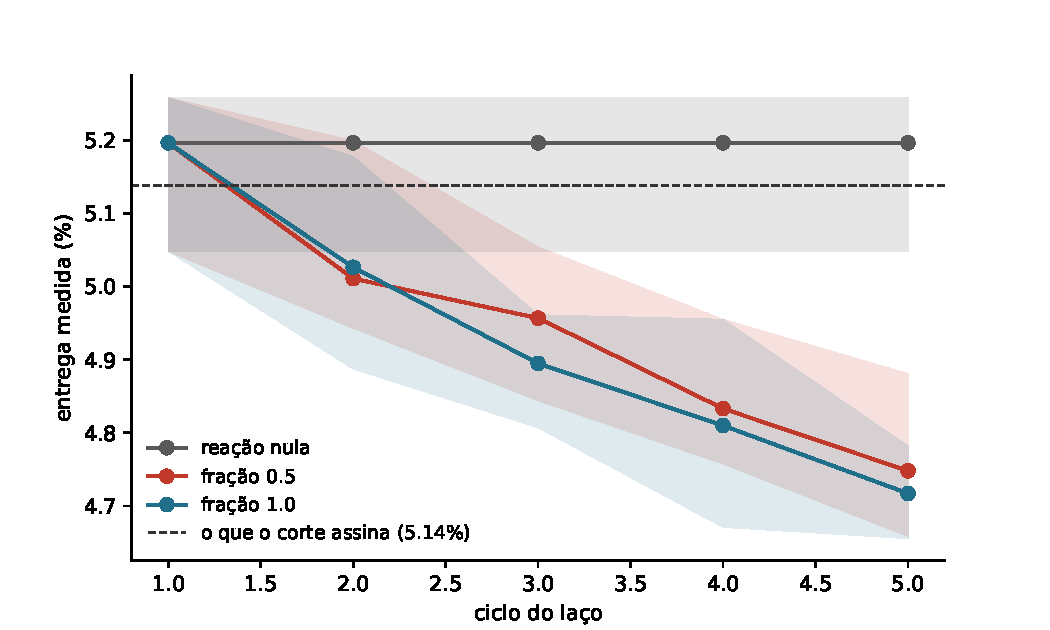
\includegraphics[width=\textwidth]{figuras/E35_performativos_1.pdf}
\caption{A entrega ciclo a ciclo quando a venda cai no próprio dia do rompimento (atraso zero):
mediana entre mundos e faixa dos vinte aos oitenta por cento, para a reação nula e as duas
frações vendidas, contra a linha do que o corte assina. A reação puxa a entrega para baixo ciclo
a ciclo; a faixa entre mundos mal se estreita.}
\label{fig:laco_entrega}
\end{figure}

Vender no dia do rompimento é real. A entrega cai de \numLacoEntregaNulaMedianaPct\% para
\numLacoEntregaFracaoInteiraAtrasoZeroMedianaPct\%: a diferença pareada por mundo é de
\numLacoDiferencaInteiraAtrasoZeroMedianaPct\% contra a dispersão de
\numLacoDiferencaInteiraAtrasoZeroDispersaoPct\% --- quase quatro vezes o ruído entre mundos. O
laço existe: o instrumento conversa, e a conversa muda a entrega.

Um dia de atraso desarma tudo. Com a venda marcada para o dia seguinte, a diferença cai para
\numLacoDiferencaFracaoInteiraMedianaPct\% contra a dispersão de
\numLacoDiferencaFracaoInteiraDispersaoPct\%: o tamanho do ruído. A razão é estrutural, e é a
mesma que o capítulo vai explorar na seção seguinte: o corte lê os piores dias da janela, e a
venda do dia seguinte não toca o dia que rompeu --- toca um dia que provavelmente não está entre
os piores. A reação aterra onde a estatística não olha. Quem mede durante o mundo que se move
precisa saber disso de antemão \cite{mendlerdunner2020stochastic}: o atraso da reação decide se o
instrumento vê o próprio efeito, antes de qualquer convergência.

\section{Meia venda e venda inteira compram o mesmo corte}

A fração não compra gradiente. No atraso de um dia, vender metade e vender por inteiro dão o
mesmo número na quarta casa: o corte anda \numLacoCorteAndouFracaoInteiraPct\% com a fração
inteira e \numLacoCorteAndouMeiaFracaoPct\% com a metade --- iguais, contra a dispersão de
\numLacoCorteAndouFracaoInteiraDispersaoPct\% entre mundos. A razão é a ordem: o corte é o
décimo terceiro pior, estatística de posição, não de magnitude. Qualquer amortecimento forte o
bastante para tirar o dia da lista dos piores deixa o próximo da fila no lugar dele, e o corte lê
o próximo --- o mesmo valor se sair metade ou sair inteiro. O instrumento mede escalões, e o
escalão não tem meio.

É aqui que a pergunta da estabilidade performativa \cite{perdomo2020performative} ganha a resposta
desta família: o ponto em que a recalibragem para de se mover é alcançado numa volta só, e não por
convergência --- é cegueira da ordem. O laço de um dia de atraso não converge; ele simplesmente
não é visto.

\section{O corte que anda}

No atraso zero, onde a reação é vista, o corte não converge --- anda. A mediana entre mundos começa
em \numLacoCorteCicloPrimeiroFracaoInteiraAtrasoZero{} e termina, cinco ciclos depois, em
\numLacoCorteCicloQuintoFracaoInteiraAtrasoZero{}: um movimento de
\numLacoCorteAndouFracaoInteiraAtrasoZeroPct\% contra a dispersão de
\numLacoCorteAndouFracaoInteiraAtrasoZeroDispersaoPct\% entre mundos, monotônico ciclo a ciclo
--- \numLacoCorteCicloSegundoFracaoInteiraAtrasoZero{},
\numLacoCorteCicloTerceiroFracaoInteiraAtrasoZero{},
\numLacoCorteCicloQuartoFracaoInteiraAtrasoZero{} --- e ainda andando na quinta volta. Cinco
ciclos não bastam para dizer onde ele para.

A leitura é a performatividade em câmera lenta: a venda amortece os extremos, o corte seguinte lê
um mundo mais calmo e sobe, a barra mais alta encontra dias mais leves, e a entrega cai um pouco a
cada volta. O instrumento certifica a calma que a própria ação criou --- a medida e o medido
andam juntos \cite{perdomo2020performative}. E a decisão que conta o próprio efeito é a única que
não erra sempre para o mesmo lado \cite{miller2021outside}: aqui o corte que sobe é o efeito da
venda ser contada na série, não um mundo que ficou mais gentil por conta própria.

\section{O preço, na moeda da partilha}

\begin{figure}[ht]
\centering
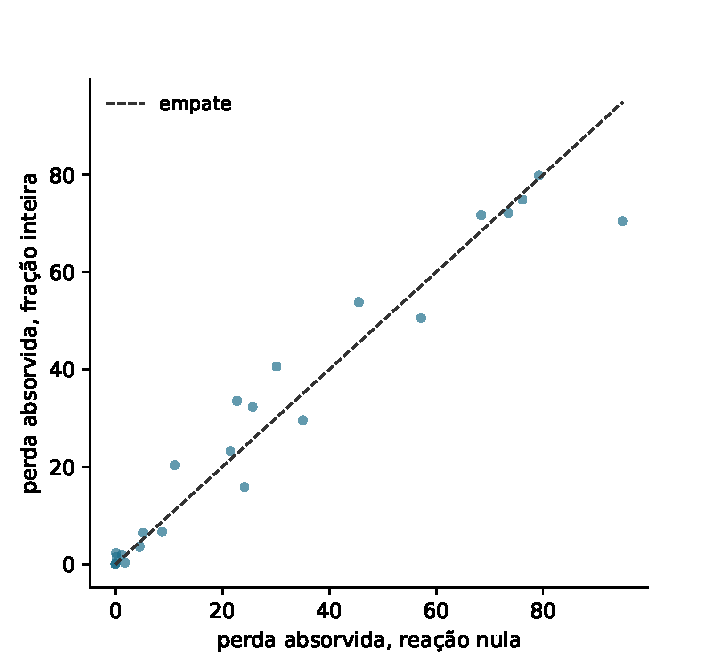
\includegraphics[width=0.72\textwidth]{figuras/E35_performativos_2.pdf}
\caption{O preço pareado por mundo: a perda absorvida com a venda inteira no dia do rompimento
contra a da reação nula, um ponto por mundo, na diagonal de empate. Os pontos caem onde a
dispersão entre mundos manda: o efeito que a entrega vê é do tamanho do ruído na moeda da
partilha.}
\label{fig:laco_preco}
\end{figure}

Resta a conta que o capítulo da partilha deixou: a moeda dela, a perda absorvida. No mesmo
orçamento de atualizações, a reação inteira no dia do rompimento absorve
\numLacoPrecoAbsorvidoFracaoInteira{} contra \numLacoPrecoAbsorvidoNula{} da reação nula --- uma
diferença mediana de \numLacoPrecoDiferencaInteiraMediana{} contra a dispersão de
\numLacoPrecoDiferencaInteiraDispersao{} entre mundos. Empate. O efeito que a entrega enxerga
quase quatro vezes o ruído é invisível na moeda da carteira: a venda muda o que o vigia lê, e não
muda o que a barreira deixa passar, nesta família e neste orçamento. A proposição declarava que o
empate também é resposta, e é a que fica: para o preço, o laço é do tamanho do ruído.

\section{O que fica}

O capítulo abriu com a decisão de agir no disparo e termina com ela medida. A ação só existe para
o instrumento quando cai no dia do rompimento --- um dia de atraso e a estatística de ordem
engole a reação sem deixar recibo. Quando existe, ela anda com o corte, que sobe certificando a
calma que a própria venda fabricou. E para a carteira, nesta família, ela não paga nem custa: o
empate está declarado com a dispersão junto.

Sobra a outra metade do limite que a partilha mediu. A escala é a que precisa ser atualizada
sempre, e o capítulo mostrou o que a atualização faz quando o mundo reage; falta o que ela faz
com o passado --- atualizar é esquecer, e quanto do passado se pode apagar antes que o sistema
deixe de aprender é a conta que o capítulo seguinte paga.